\chapter{Results}

In this chapter speed measurements of our application will be presented as well as few pictures of results.
Because we have not speedup the computation over traditional processors discussion of the reasons will follow the results.
We will mention possible changes in design to speed up the execution.
Then some consideration how shall look the algorithm that is well suited for Cell B.E. like.
Chapter will be finished with comparison of complexity of programming for Cell B.E. and conventional processors.

\section{Speed measurements}

\par
Actual speed measurement is performed within \emph{GenerateData} method of the FiniteDifferenceFilter.
Counter is started right after initialization phase (i.e. before main algorithm loop) and stopped right after the loop.
Program memory usage was tuned to use only really necessary amount of memory within measured interval.
Valgrind's massive tool was used for the memory usage tuning.
This was necessary because of the PS3 small memory and because we want to leave swap file untouched during the speed measurement.

\par
Meanwhile this server memory usage tuning some changes was made also within client part.
There was special filter developped.
That filter shrinks data set to given size and cast its voxels to float.
Shrinking is performed by linear interpolation.
The purpose of the float casting is avoiding allocation of additional memory to perform it on the server side.

\par
It is strange that command top shows far bigger memory usage than Valgrind's massif.
We have not care much about it but the idea is that top shows all memory requested from system while massif shows exact memory used by process.

\par
Results of the speed measurement is summarized within Table \ref{tab:runresults}.
Every measurement was run with the same curvature and speed-scaling factors.
But with different initial distance, maximum iterations and seed parameters.
These parameter was set according data set size.

Three different data sets were measured.
All of them was CT images of skull.

\begin{table}
\centering
\begin{tabular}{|c|c|c|c|c|c|c|}
\hline
\multicolumn{7}{|c|}{Measurement results}\\
\hline
data set		&size		&seed		&init.		&max. 		&arch.		&time\\
			&		&		&dist-		&itera-		&		&spend\\
			&		&		&ance		&tions		&		&(sec)\\
\hline
\hline
3slices 		&512x512x3	&[256,256,1]	&40		&800		&Cell B.E.	&16.48\\
(skull 1)		&512x512x3	&[256,256,1]	&40		&800		&i686	.	&1.89\\
\hline
\hline
skull 1			&256x256x80	&[128,110,20]	&20		&500		&Cell B.E.	&471.89\\
			&256x256x80	&[128,110,20]	&20		&500		&i686		&95.23\\
\hline
\hline
skull 1			&256x256x80	&[128,110,20]	&4		&500		&i686		&61.74\\
\hline
\hline
skull 2			&256x256x80	&[128,110,20]	&4		&500		&i686		&55.88\\
\hline
\hline
skull 2			&256x256x80	&[128,128,40]	&4		&500		&i686		&76.9\\
\hline
\end{tabular}
\par
\caption[Measurement results]
{
  Results of speed measurement //TODO
}
\label{tab:runresults}
\end{table}

\section{Pictures}

\section{Reasons of slowdown and possible improvements}

\par
Porting the code to run on SPEs is not sufficient to get more speed from Cell B.E. over traditional processors.
Additional speedup porting phases are necessary.
But our program has another speed pitfalls.

\par
The biggest of them is CellNeighbourhood that represent small segment of an image (the $3^3$ voxel matrix).
It is transferred for every layer (linked chain of nodes) item.
In some parts the both output and status image neighborhoods are transferred.
We wanted to perform the transfer in scatter-gather manner through the DMA lists but we have faced some problems concerning this way of transfer.
The DMA transfers (and specially using DMA lists) are designed for bigger amount of aligned data.
When used for small amounts (smaller that 16bytes per list item) performance goes down because transfer of unaligned data.
When data smaller than 16 bytes (quad-word) are being transferred, every single item is automatically aligned to quad-word address within local store buffer (see Figure \ref{fg:automaticAlignOfSmallData}).

\begin{figure}
    \centering
    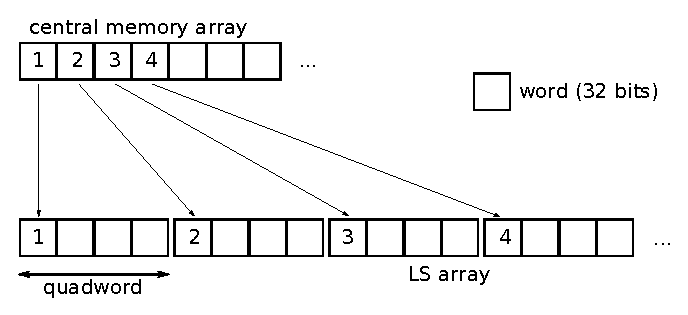
\includegraphics[width=0.8\textwidth]{data/automaticAlignOfSmallData}
    \caption[automatic align of small data]
{
  Illustration of transfer of data that are smaller that quad-word.
  Hardware automatically increase address within local store buffer in such way that every transferred item is quad-word aligned.
}
    \label{fg:automaticAlignOfSmallData}
\end{figure}

This increase required size of buffer that is needed for the transfer.
This can be partially solved by usage of multiple DMA lists (one for each quadword align).
This is illustrated on Figure \ref{fg:multipleDMAList}.
For details see \cite{DMAListIssues}.

\begin{figure}
    \centering
    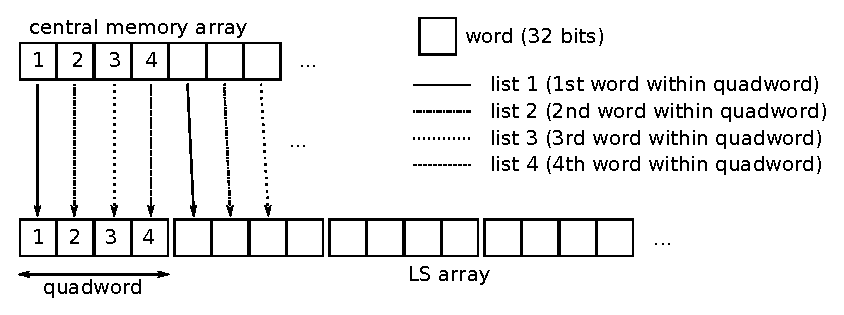
\includegraphics[width=0.95\textwidth]{data/multipleDMAList}
    \caption[multiple DMA list workaround]
{
  Workaround for transfer in smaller than quad-word chunks.
  Uses more that one DMA list.
  One per quad-word align (e.g. for single bytes 16 DMA lists are needed).
}
    \label{fg:multipleDMAList}
\end{figure}

We have adopted this workaround and used it within the neighborhood transfer.
Because if automatic local store quadword address aligning we had to use a translation table that maps position of actual neigbourhood members into the local store buffer which had to be enlarged appropriately based on data type that stores.
This is working solution but overhead for SPE is incredible and thus useless (see cellNeigbourhood.tcc for details).

\par
\label{neighbourhoodDependecy}
Another problem is order of layer nodes (and thus neighborhoods) processing.
When there are two nodes within one layer that are next to each other and processed subsequently.
Changes made to the first processed neighborhood would not appear to already preloaded next one.
So another merging need to be performed.

\par
This coerced another changes to neighborhood transfer and made the actual transfer unbearably expensive operation.

\par
\label{workDependecy}
Additional pitfall is the situation when sibling nodes are processed by two different SPEs.
Adding nodes to layers is based on information from currently processed node's neighbors.
So it is possible that two different SPE inserts the same nodes more time into one layer because they process sibling nodes (i.e. overlapping neighborhoods).
This makes no changes to output but additional overhead due to processing multiplied nodes.
Solution to this problem would be synchronization among the SPEs.

\par
To speed up the execution improvement of neighbourhood transfers should be done.
This corresponds to data transfer optimization step of porting process (see \ref{fg:appPorting})
In our case this means radical simplification of neighborhood transfers.
This transfers should take only a few instructions to be effective.
Within SDK examples they are performed by simple macros which is probably the most effective way.
In our case simplification if the neighborhood transfer would mean utilization of bigger image parts transport within the DMA transfers to avoid automatic local store alignment for small data transfers.
This would mean a bigger local store array to store the image part but processing of nodes that are associated with the part would be somehow gathered and thus the count of transfers would be less.
Processing of nodes should take into account their spatial information when inserted into a layer and thus to gather the node processing on the bigger neighborhood.
But such computation scheme would coerce complete redesign of application.

\section{Code and design complexity}

\par
Cell B.E. programming means mainly programming for SPEs because of their performance and count.
Because of indirect memory access and need of usage of some multi-bufferring memory transfer scheme the design is quite more complex over common processor.
With another limitation which is the local store size is design of Cell B.E. application a challenge.

\par
Cell B.E. is designed for intensive computation programs.
For programmer this means utilize all SPEs and all their features at maximum level.
It is only possible for certain class of algorithm.
Lets call them streaming parallel algorithm.
But what is it? What is the definition?
Work on our application has showed us what is not the streaming parallel algorithm.
So by negation of features that slow down our program we could get definition of such streaming parallel algorithm:
\begin{enumerate}

\item{Streaming nature}
\par
Data of that program are uniform and can be processed in small pieces (chunks) which are mutually independent which can fit in local store memory.
This means that for one chunk processing is only necessary this chunk and not any part of other chunks.
And when this chunk is once processed is stored and never retrieved for processing again.

\par
For our application this is not true.
At least not for all the input data.
Processing of a sparse field layer (linked chain of nodes) meets the streaming nature.
But processing of parts of underlying images (neighborhoods) associated with this nodes does not.
Neighbourhoods are mutually dependent see \ref{neighbourhoodDependecy}.

\item{Paralel nature}
\par
Input data can be divided into parts which are again mutually independent and which can be sent to particular cores for processing.

\par
For our application is again not true.
Work that is divided among the cores is not independent because of dependency of particular neighborhoods.
See \ref{workDependecy} what causes problems.

\end{enumerate}

\par
When algorithm does not meet the streaming parallel definition then it should not be implemented or changed.
This means e.g. to use different data structures.
In our case, change of the data structure to somehow gather node processing to specific image part would be the change of algorithm we implemented leading to performance gain.
But then this would be the original algorithm any more.

\par
In contrast there are algorithms that fits the streaming paralel algorithm definition.
Among the examples within SDK e.g. thresholding is one of them.
It operates on image that has uniform data - pixels.
It apply simple condition on each pixel which result depends only on the processed pixel.
Processing can be divided into chunks.
These three features meets the streaming condition.
Moreover the data can be divided into independent sets that can be processed by multiple cores (the parallel nature).
Implementation of this algorithm can therefore result huge performance gain on Cell B.E. than conventional processors.

\par
Our work has showed importance of initial consideration and design phase.
When there is more algorithms that are solving desirable problem programmer should think carefully which one will be the best for porting to Cell B.E.
First stage of the initial consideration should be model of the application implementing chosen algorithm.
Thing what kind of data are processed.
If they are uniform.
If they are divisible into chunks.
If the computing can be divided into independent parts i.e. what entity defines amount of work to be done.
These are question that leads to answer if the chosen algorithm is or is not the streaming parallel.
If the answer is no, implementation of that algorithm is rather worthless and will result such suboptimal program as the ours.

\par
Another thing is the code complexity.
Performing the optimisation porting cycle steps utilise leanguage intrinsics for differend kind of special instructions usage of macros for variety of purposes.
These techniques increase actual code complexity whereas may decrease code readability.

\subsection{Algorithm complexity}

\par
There is still another question to be answered.
Is implementation of an algorithm worth at all?
Since only some special products is equipped with Cell B.E. actual data has to be sent to such mashine for computing and results has to ber sent back.
So only complex algorithm where performance gain would be bigger than the time spent in transfer of actual data set are worth to port.
The algorithm we have tried to implement is complex enough to be offloaded to compute on remote machine while the mentioned thresholding would not.
As soon as common machines such as notebooks, desktops are equipped with the Cell B.E. processor even class of such simple image processing algorithms that is implemented in everyday-use software (such as the thresholding or variety of masking, edge detections) could take advantage of the processor.

\chapter{Conclusion}

At the beginning we studied available literature to find out what is actually Cell B.E., what benefits it brings for what price.
What special features it have and what are they good for.
Then we have been trying to install SDK to start actual development process.
During this phase we faced some obstacles like bugs, incompatibilities among tools, libraries that the tools use and even operating system vs. SDK incompatibilities.
So we had to go through variety of forums and other sources to find the solution.
As a side effect we improved our Linux knowledge.
Eventually we managed to install SDK and was able to start developing.
Then we tested variety of libraries, tools and other feature that the SDK brings.
We have chosen sparse field algorithm implementing level set based segmentation to port to Cell B.E. platform.
This is quite complex algorithm to test the platform's potential.
We adopted ITK implementation of that algorithm.
So we had to study ITK toolkit and its internals.
We have also incorporated the whole program into MedV4D framework.
That means we have implemented some new modules that allows using ITK and can offload some part of processing to another machine (that run on Cell B.E.).
Actual porting process started with profiling of existing application.
This step have found out hot spots of the code which can be in turn offloaded to SPE to take advantage of Cell B.E. potential.
But results was quite unexpected so another redesign of application followed.
In this new design almost whole original ITK pipeline was offloaded into SPE.
Big code restructuring was necessary to allow to perform actual computations on SPE.
Finnaly we have able to run the whole algorithm on SPE and thus to measure time need for computations.
The result of measurement showed that simple move the computation to SPE slows down the computations because of insufficient utilization of Cell B.E. features.
We have identified some bottlenecks of the application and discussed possible solutions.
Implementation of these solutions would require whole application redesign using another data structure.
This changes would actually mean change of used algorithm.

\par
We have also discussed differences between programming conventional processors and Cell B.E.
As well as question of actual algorithm complexity and worthiness of porting them to Cell B.E.


\par
The Cell B.E. platform is very interesting for its variations of use scenarios and ability of program tuning and customization.
We think the pallet of tools and features of the Cell B.E. can make it interresting alternative to conventional processors whose lifetime gets shorter due to limitations in manufacturing process.
Cell B.E.'s great potential has already been proven but it is still waiting for wider spectrum of programmers.

\par
If the process of starting developing on Cell B.E. would become simpler we believe much more new programmers would be start.
Nowadays there are plenty of information about Cell B.E. but somehow unsorted or out of date.
The best information source are documents shipped along the SDK.
But they are targeted to contain all the information regardless the level of experience of the reader.
So when a programmer wants to start developing applications on Cell B.E. he would go trough plenty of that information before he can start actual work.
It's a pity there are total lack of information for PS3 users within SDK docs.
This is quite problem when big part of beginners has PS3 available.
There is simply lack of some "cookbook for beginners" with practical information and some howtos.
We believe is such cookbook with some of practical information that potentially may help to some other programmers who would like to start developing for Cell B.E.